%% -*- coding:utf-8 -*-
\documentclass[ number=??
                ,series=lnls,
                ,isbn=xxx-x-xxxxxx-xx-x,
                ,url=http://langsci-press.org/catalog/book/14,
	        ,output=long    % long|short|inprep              
	        %,blackandwhite
	        %,smallfont
	        ,draftmode  
		  ]{langsci}                          

          
\hypersetup{pdfdisplaydoctitle=true}

\usepackage{xspace}
\newcommand{\latex}{\LaTeX\xspace}



% just for the XeLaTeX logo
\usepackage{dtklogos}\newcommand{\xelatex}{\XeLaTeX\xspace}
\newcommand{\bibtex}{\BibTeX\xspace}

\usepackage{lsp-makros}

\usepackage{german}\selectlanguage{USenglish}

\usepackage{lsp-eng-hyp}

\usepackage{abbrev}


% AVMs
\usepackage{lsp-styles/avm}
\avmfont{\sc} 
\avmvalfont{\it}
      
% OT pointing hand
\usepackage{pifont}
\newcommand{\hand}{\ding{43}}

% OT tableaux                                                
\usepackage{pstricks,colortab}   

% DRS package by Alexis Dimitriadis
%\usepackage{drs}

\usepackage{tabularx}


\usepackage{tikz-qtree}
% has strange side effects
%\tikzset{every tree node/.style={align=left, anchor=north}}
\tikzset{every roof node/.append style={inner sep=0.1pt,text height=2ex,text depth=0.3ex}}

\usepackage{jambox}
 
\usepackage{lipsum}  

\setlength{\marginparwidth}{1.5cm}
\usepackage[textsize=tiny,textwidth=1.5cm]{todonotes}
\newcommand{\todostefan}[1]{\todo[color=green!40]{#1\xspace}}
\newcommand{\inlinetodostefan}[1]{\todo[color=green!40,inline]{{\normalsize #1}}}


% Chinese
\usepackage[indentfirst=false]{xeCJK}
\setCJKmainfont{SimSun}

% bidirectional text and support for Arabic/Persian
%% \usepackage{fontspec}
\newfontfamily\Parsifont[Script=Arabic]{XB Niloofar}
%\usepackage{bidi}
\usepackage{lsp-bidi}
\newcommand{\PRL}[1]{\RL{\Parsifont #1}}
%\TeXXeTOff
\usepackage{lsp-gb4e}



\title{How to Write a Book for Language Science Press}  
\subtitle{Guidelines for Authors and \latex Recommendations}
\BackTitle{How to Write a Book for Language Science Press}
\BackBody{This book contains the guidelines for Language Science Press authors. For those who want
  to help keeping the production costs low and therefore decided to use \latex it also contains
  descriptions of packages that can be used for typesetting trees, Attribute Value Matrices, OT-tableaux, Categorial
  Grammar proofs, LFG analyses, and much more. The setup of typesetting script with special fonts as
  for instance right to left scripts like Arabic is explained. The \latex chapter also contains sections
  concerning the efficient workflow in professional typesetting environments using \latex.

Stefan Müller is an experienced \latex user who has typeset four published books and several book
manuscripts and journal articles.
}

\dedication{This book is dedicated to everybody who cannot afford to buy books by profit oriented publishers.}

\author{Stefan Müller}



\makeatletter
\def\verbatim@font{\scriptsize\ttfamily}
\makeatother
         
%\renewcommand{\eachwordone}{\it}
%\renewcommand{\exfont}{\it}
%\def\exfont{\it}

\begin{document}               
         
                                                                           
                                  
\maketitle                

%\frontmatter

\chapter*{Preface}

%\lipsum[3-10]  

The purpose of this book is twofold: it contains a guideline with some style recommodations for all
authors. The second part is for authors who use \latex or who want to learn \latex in order to
support \lsp. The second part is also a reference for those who volunteered to help typesetting
manuscripts that were not submitted in \latex. See \citew{MuellerOA} and \citew{MH2013a} for an overview of the
general setup of the project.

\section*{Acknowledgements}



%% David Reitter danke ich für die \LaTeX"=Makros für Combinatorial
%% Categorial Grammar, Mary Dalrymple und Jonas Kuhn für die LFG"=Makros und Beispielstrukturen, und
%% Laura Kallmeyer für die \LaTeX"=Quelltexte der meisten TAG"=Analysen. Ohne diese
%% Originalmakros/-texte wären die Darstellungen in den jeweiligen Kapiteln sicher nicht halb so schön
%% geworden. 

This book is typeset with \xelatex. We thank the \latex developers for their work and the members of the German \textit{German
  Language TeX Users Group Communication List} and those replying at \url{http://tex.stackexchange.com} for many usefull hints and suggestions.

I thank Matthias Hüning\aimention{Matthias H{\"u}ning} for comments on an earlier version of this document and Corinna Handschuh\aimention{Corinna Handschuh}
and Francesco Cangemi\aimention{Francesco Cangemi} for being the first ones using the new \latex classes and providing feedback
to us.

\bigskip

\noindent
Berlin, \today\hfill Stefan Müller


\tableofcontents      

\mainmatter         

%% -*- coding:utf-8 -*-
\chapter{General Information on Language Science Press}

\section{Background and Motivation}

\section{Set Up and Responsibilities}

\subsection{Advisory Board}

\subsection{Series and Editorial Boards}

\subsection{Open Monograph Press and ZEDAT/CEDIS}

\subsection{The Library of the Freie Universität Berlin}



%% -*- coding:utf-8 -*-
\chapter{Guidelines for authors}

The following sections describe the layout of various items that play a role in typesetting. 

\section{Headings}

Please provide the headings of chapters and sections in normal spelling. If you are writing English,
please do not capitalize content words unless capitalization is required by orthographical rules. 

Your document may use structures up to six levels, that is there may be a section with
the number 1.2.3.4.5.6.\footnote{
  See page~\pageref{sec-Chinese} for an actual use of subsubsections.%
} However, such elaborated structures may be difficult for the readers, so
there should be a good motivation for going beyond four levels.

%\subsubsubsubsection{Test}

\section{Emphazizing}

If you want to \emph{emphazize} terms, please use \emph{italics}. Bold face has to be avoided under
any circumstances. The only place where boldfase is used is section headings.

\section{Glossed examples}

Please gloss all examples and provide them with translations. The glossing should be done according
to the Leipzig Glossing Rules. If you need special abbreviations that are not defined by the Leipzig
Glossing Rules\footnote{
\url{http://www.eva.mpg.de/lingua/resources/glossing-rules.php}. 27.10.2013.
}
\todo{Martin: provide an example}, put them in a table immedeately before the first chapter of a
monograph. In case of edited volumes the tables with abbreviations should be placed immedeately
before the references.

\section{Figures and tables}

Figures and tables should come with a caption. Captions are set below figures and above tables. The caption should be in
normal spelling, that is without capitalization of content words. Please number figures and
tables. The number should consist of the chapter number and a number that starts with one for every
new chapter. There has to be one counter for figures and another one for
tables. Figure~\vref{fig-example-fig-the-dog-barks} is an example of a figure and
Table~\vref{tab-example-croft} is an example of a table.

\begin{figure}[htbp]
\centerline{%
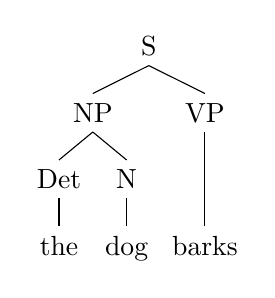
\begin{tikzpicture}
\tikzset{level 1+/.style={level distance=2\baselineskip}}
\tikzset{frontier/.style={distance from root=6\baselineskip}}
\Tree[.S
       [.NP 
         [.Det the ]
         [.N   dog ] ]
       [.VP barks ] ]
\end{tikzpicture}
}
\caption{\label{fig-example-fig-the-dog-barks}An example of a figure: Analysis of the sentence \emph{The dog barks.}}
\end{figure}

\begin{table}[htbp]
\caption{\label{tab-example-croft}An example of a table taken from \citew[214]{Croft2003a}}
\centerline{
\begin{tabularx}{\textwidth}{llX}\hline\hline
          & Low categoriality unit      & Unit with wich it clusters\\\hline
`Noun'    & low referentiality NP       & forgrounded verb\\
          & attached body part noun     & forgrounded verb\\
          & anaphoric NP                & forgrounded verb, emphasized element\\
`Verb'    & tense/aspect/mood auxiliary & forgrounded verb\\ 
\hline\hline
\end{tabularx}
}
\end{table}

\section{Footnotes}

Please use footnotes rather than endnotes. Footnotes go to the end of the clause after punctuation
unless they refer to a specific word or phrase.\footnote{
  This is an example of a footnote that refers to the whole clause.
}

Please do not use footnotes in tables or figures\footnote{
  This is a footnote that refers to the word \emph{figures}. If only there was something interesting
  to say about figures apart from the fact that they are floating objects.
} but attach them to the text preceeding or following them.


\section{Quotations}

If long passages are quoted, they should be indented and the quote should be followed by the exact reference:
\begin{quotation}
Precisely constructed models for linguistic structure can play an
important role, both negative and positive, in the process of discovery 
itself. By pushing a precise but inadequate formulation to
an unacceptable conclusion, we can often expose the exact source
of this inadequacy and, consequently, gain a deeper understanding
of the linguistic data. More positively, a formalized theory may 
automatically provide solutions for many problems other than those
for which it was explicitly designed. Obscure and intuition-bound
notions can neither lead to absurd conclusions nor provide new and
correct ones, and hence they fail to be useful in two important respects. 
I think that some of those linguists who have questioned
the value of precise and technical development of linguistic theory
have failed to recognize the productive potential in the method
of rigorously stating a proposed theory and applying it strictly to
linguistic material with no attempt to avoid unacceptable conclusions 
by ad hoc adjustments or loose formulation.
\citep[5]{Chomsky57a}
\end{quotation}
%
Short passages should be quoted inline in italics: \citet[5]{Chomsky57a} stated that \emph{[o]bscure
  and intuition-bound notions can neither lead to absurd conclusions nor provide new and
correct ones}.

If you quote text that is not in the language of the book provide a translation. Short quotes should
be translated inline, long quotes should be translated in a footnote.

\section{Crossreferences in the text}

Please use the crossreferenceing mechanisms of your text editing/type setting software. Using such
crossreferencing mechanisms is less error-prone when you shift text blocks around and in addition
all these crossreferences will be turned into hyperlinks between document parts, which makes the
final documents much more useful.

If you have numbered example sentence, please start with (1) for every new chapter.

Please use capitals if you refer to specific sections, tables, or figures: \emph{As we have shown in
  Section~3.1}, \emph{As Figure~3.5 shows}. Do not capitalize without a number: \emph{In the
  following section we will discuss}.\todostefan{What about footnotes? I usually do not
  capitalize. Seems inconsistent.}

\section{References}

If books or larger articles are cited, exact page numbers should be provided. This is both good for
authors since it helps them to keep track of their source and enables them to find and reread the
referenced passages and it is a good service to the readers.

We use the \emph{Unified Style Sheet for Linguistics}, which is described here:
\url{http://celxj.org/downloads/UnifiedStyleSheet.pdf}. The \bibtex file is contained in the \latex
classes that are used for typesetting \lsp books. Please deliver a \bibtex file with all your
references together with your submissions. \bibtex can be exported from all common bibliography
tools (We recommend BibDesk for the Mac and JabRef for all other platforms).

The references in your \bibtex file will be typeset correctly automatically. So, provided the
\bibtex file is correct, authors do not have to worry about this. But there are some things to
observe in the main text. Please cite as shown in Table~\ref{tab-citation}.

\begin{table}[htbp]
\caption{\label{tab-citation}Citation style for \lsp}
\centerline{%
\begin{tabular}{lp{9cm}}\hline\hline
citation type & example\\\hline
author & As \citet[215]{MZ85a} have shown\\
       & As \citet[215]{MZ85a} and \citet{Bloomfield33a} have shown\\
work   & As was shown in \citew[215]{Saussure16a}, this is a problem for theories that \ldots\\
work   & This is not true \citep{Saussure16a,Bloomfield33a}.\\\hline\hline
\end{tabular}
}
\end{table}

%% Table~\ref{tab-various-publication-types} provides examples for different publication types (book,
%% journal article, paper in an edited volume, and so on). Please refer to the bibliography at the end
%% of this book to see how the respective items are formated.

If you have an enummeration of references in the text as in \emph{As X, Y, and Z have shown}, please use
the normal punctuation of the respective language rather then special markup like `;'.

\noindent
\inlinetodostefan{Say something about decapitalization.}


\section{Edited volumes}

Papers in edited volumes should start with an abstract.


\section{Checklist}

The following is a general checklist for authors. Author who use \latex should also consult the
checklist for advanced authors/typesetters in Section~\ref{sec-check-typesetters}.



















%      <!-- Local IspellDict: en_US-w_accents -->

%% -*- coding:utf-8 -*-
\chapter{\LaTeX}

\section{Installation of the \texttt{langsci} class}

The \latex class for typesetting Language Science Press books was developed by Timm
Lichte\aimention{Timm Lichte} with
help be Berthold Crysmann\aimention{Berthold Crysmann} and me\aimention{Stefan Müller}. It can be downloded from the GitHUB\is{GitHUB} repository at: \url{https://github.com/langsci/latex}
You can download the classes directly from the given web page or use the following git commands to
create a local copy of the repository:
\begin{verbatim}
git init
git clone https://github.com/langsci/latex.git 
\end{verbatim}
If you are using \texttt{git}, you can update your installation by executing the following command:
\begin{verbatim}
git pull origin
\end{verbatim}

Place all files and subdirectories from this repository into your local working directory.

\section{Using the \texttt{langsci} class}

Once you installed the classes in your system, you may look at the file \texttt{test.tex} to see how
a book can be typeset. The code of this book is available in the directory \texttt{Guidelines}. Once
you set up your \latex files you can compile them by calling 
\begin{verbatim}
xelatex yourfilename.tex
\end{verbatim}

%\DescribeMacro{\BackTitle}


\subsection{Class options}

A \latex document starts with a specification of a document class. Usually this is a class for
books, articles, or technical reports. \lsp has a special class that is called \texttt{langsci} and is
based on the book class from the KomaScript package. Several options can be passed to the class. The
following code shows how the class is loaded and how options are set. 


\begin{verbatim}
\documentclass[series=labphon,
               number=1,
               isbn=978-3-944675-01-5,
               url=http://langsci-press.org/catalog/book/16,
               output=long]{langsci}            
\end{verbatim}

The options are explained in the following paragraphs.


\subsubsection{\texttt{series}}

The\isoption{series} name of the series in which a book is published has to be passed to the langsci package. This will ensure that the name of
the series is put on the cover and the right color for your series will be
selected. Table~\vref{table-series} provides an overview of the series that are established as of
\today.
\begin{table}[htbp]
\caption{\label{table-series}Series of \lsp as of \today}
\centerline{%
\begin{tabular}{ll}\hline\hline
Option  & Full Name\\\hline
eotms   & Empirically Oriented Theoretical Morphology and Syntax\\
eotmsig & Implemented Grammars\\
sidl    & Studies in Diversity Linguistics\\
algad   & African Language Grammars and Dictionaries\\
tmnlp   & Translation and Multilingual Natural Language Processing\\
lnls    & Lecture Notes in Language Sciences\\
nc      & Monographs on Comparative Niger-Congo\\
labphon & Studies in Laboratory Phonology\\
\hline\hline
\end{tabular}
}
\end{table}



\subsubsection{\texttt{number}}

Authors\isoption{number} will be informed by their editor about the number that their book has in the series. This
number is passed with the \texttt{number} option to the langsci class.

\subsubsection{\texttt{isbn}}

Once\isoption{isbn} a manuscript is accepted, authors have to sign a publication agreement with the FU Library (see
Chapter~\ref{chap-publication}). Then they will get an ISBN, which has to be passed to the langsci class.

\subsubsection{\texttt{url}}

When\isoption{url} a manuscript is submitted to \lsp the submission gets a number and there will be a
corresponding URL. This URL has to be passed to the langsci class, since it will be part of the
impressum of your book.

\subsubsection{\texttt{output}}

There\isoption{output} are three options for output: \texttt{long}, \texttt{short}, and \texttt{inprep}. If you pass
\texttt{long} to the langsci class, all pages are printed. This includes front and backpane of the
cover and also its spine. If the option \texttt{short} is used, the cover pages are omitted. This
document version is much more printer friendly since the colored pages are not included.

The option \texttt{inprep} suppresses everything that refers to \lsp. This gives authors the
possibility to write their book using the \lsp classes and styles prior to submission. They may then
distribute the manuscript without revealing their intention to submit to \lsp.

\subsubsection{\texttt{smallfont}}

\lsp\isoption{smallfont} books are typeset with an 11pt font. Those books that would be longer than 500 pages should be
typeset with the \texttt{smallfont} option, which selects a 10pt font.

\subsubsection{\texttt{draftmode}}

Since\isoption{draftmode} \lsp does not have any commercial interest you can put your book on webpages and distribute it
freely. We encourage authors to do this in order to discuss the work and improve it before final
publication. If authors want to circulate prefinal versions, they can use the option
\texttt{draftmode}. This prints a large watermark onto the first page and adds a footer to ever page
that informs the reader about the fact that he is reading a draft and the date and time of the
creation of the draft.




\subsection{Commands}

You can specify a title with the \verb+\title+\iscommand{title} command (\latex standard). In addition the langsci
class provides a command for specifying a subtitle (\verb+\subtitle+\iscommand{subtitle}). The author of a book is
specified by \verb+\author+\iscommand{author}. A separate page with a dedication can be inserted by \verb+\dedication+\isoption{dedication}.

The title of the book that goes to the back of the book is specified by \iscommand{BackTitle}\verb+\BackTitle+ and the
cover text on the back is provided by \verb+\BackBody+\iscommand{BackBody}.


\section{Workflow}

\subsection{Compiling the document}

\subsection{Makefiles}

\subsection{Using includes}

\subsection{Version control}


\section{Document structure}




\subsection{References}

\lsp uses the \texttt{natbib}\ispackage{natbib} package together with \bibtex\is{bibtex@\bibtex} and the \bibtex style \texttt{unified.bst}.

\subsection{Crossreferencing}

You may use \verb+(\mex{1})+\iscommand{mex} to refer to the following example and \verb+(\mex{0})+ to the preceeding
example. You can also pass smaller numbers or larger numbers to \verb+\mex+ but I would suggest not
to do this since often text blocks are inserted between the example and its description and then
references are broken. Furthermore the standard referencing mechanism creates hyperlinks to the
example sentences and depending on your viewer this gives you a nice preview of the referenced
material, which you do not get with \verb+\mex+. See Figure~\vref{fig-preview-of-hyperlink-with-skim} for an example for such a preview.
\begin{figure}[htbp]
\includegraphics[width=\linewidth]{crossref.png}
\caption{\label{fig-preview-of-hyperlink-with-skim}Hyperlinked reference allow a preview in some viewers}
\end{figure}


There should not be a linebreak in something like \emph{Section~4}. This is achieved by using an explicit
whitespace: \verb+Section~\ref{sec-examples}+ This also makes sure that \latex is not inserting too
much space when material is distributed in a line.

\subsection{Indexes}

The\is{index|(} \lsp class is set up in a way that an author index is created automatically. If you want to add
an author that is not cited (for instance in the acknowledgements), you can do this by calling
\verb+\aimention{Zappa, Frank}+.\aimention{Zappa, Frank}\iscommand{aimention}

You may enter items into the subejct index by calling \verb+\is+, for example 
\begin{verbatim}
\is{word}
\end{verbatim}

Regions can be specified by appending \verb+|(+ to the keyword at the beginning of a region and
\verb+|)+ at the end of the region. For instance this section has the index entry
\verb+\is{index|(}+ after the first word of this section and \verb+\is{index|)}+ at the very end of
this section. If this rather brief section happens to be set on one page, \latex enters one page
number into the index. If there is a pagebreak in the middle of this section, a region is entered
into the index.

If you mention a language, you may add it to the language index: 
\begin{verbatim}
\il{Mandarin Chinese}
\end{verbatim}
If you are working in a theory that uses features (like LFG or HPSG), you may use \verb+\isfeat+ to enter
features into the subject index. \verb+\isfeat{comps}+\isfeat{comps} would enter the \compsf into the subject
index. The typesetting of the feature name in {\sc small caps} will be done automatically.

All index entries are hyper-linked to the respective pages.

While working at a manuscript it can be practical to see index entries in the margins. Index entries may be
switched on by specifying \verb+\proofmodetrue+ in the preamble of the
document.\iscommand{proofmodetrue} The following specification checks whether the option
\texttt{draftmode}\isoption{draftmode} of the \texttt{langsci} is used and displays the index entries in the margin if
this is the case:
\begin{verbatim}
\iflsDraft
\proofmodetrue
\fi
\end{verbatim}
\is{index|)}

\subsection{Hyphenation}

There is a special draft mode that can be used for the preparation of manuscripts. It can be enabled
by passing the option \texttt{draftmode} to the langsci class. In draftmode words that could not be
hyphenated automatically stick out in the right margin. Such problematic words are marked with a
black box so that they can be detected easily. You can fix such problems by inserting explicit
hyphenation rules in a word. This is done by \verb+\-+, for example \verb+weath\-er+. However, this
method is dispreferred since it only affects one occurance of the word rather than all occurences in
the current and further documents. The right way to deal with hyphenation issues is to put your
hyphenation preferences into a file and include this file in all your publications. 

\begin{verbatim}
\hyphenation{
Ajd-ukie-wicz
Prze-piór-kow-ski
To-ma-sel-lo
To-ron-to
trans-for-ma-tions-gram-ma-ti-sches
Tü-bing-en
Um-welt-ver-gif-tung
Ver-lags-buch-hand-lung
West-deut-scher
Wis-sen-schaft-liche
weath-er
}
\end{verbatim}

%xxx xxxxxxxxxxxxxxxxx xxxxxxxxxxxx xxx xxxxxxxxxx xxxxxxxxxxx Wirtschaftswunder.
%
%xxx xxxxxxxxxxxxxxxxx xxxxxxxxxxxx xxx xxxxxxxxxx xxxxxxxxxxx Wissenschaftliche.



\section{Packages specific for linguistics}

There is a huge amount of packages that can be used for various purposes. \citew{MG2013a} is a good
reference book. This section discusses some aspects of some packages that are relevant for
linguistics. Every \latex package comes with a documentation and users should consult these
documentations too. The purpose of this section is to point users to the packages that we think
serve their purpose best and that are compatible with other packages and the \lsp classes, as this
book proves.

\subsection{Glossed examples}

Glossed\is{glossing|(}\ispackageb{lsp-gb4e} examples are typeset with a modified version of the \texttt{gb4e}\ispackage{gb4e} package by Craig
Thiersch\aimention{Craig Thiersch}. The modified package is called \texttt{lsp-gb4e}. It is contained in the styles directory
that is delivered with the \lsp \latex calsses. It differs from the original package in loading a
version of \texttt{gloss} that was modified by Alexis Dimitriadis\aimention{Alexis Dimitriadis} in order to be compatible with
\texttt{jambox} (see Section~\ref{sec-jambox}).

Simple examples like (\mex{1}) can be typeset as shown below.
\ea
\gll Der Mann schläft.\\
     the man  sleeps\\
\glt `The man sleeps.'
\z
\begin{verbatim}
\ea
\gll Der Mann schläft.\\
     the man  sleeps\\
\glt `The man sleeps.'
\z
\end{verbatim}
Lists of examples can be typeset with \verb+\eal+ and \verb+\zl+ respectively. The example in
(\mex{1}) shows how the sentences can be aligned properly:
\eal
\ex[]{
\gll Ich glaube dem Linguisten nicht, einen Nobelpreis gewonnen zu haben.\\
     I believe the linguist not a Nobel.prize won to have\\
\glt  `I don't believe linguist's claim that he won a Nobel prize.'
}
\ex[*]{
\gll Dem Linguisten einen Nobelpreis  glaube  ich nicht gewonnen zu haben.\\
     the linguist   a     Nobel.price believe I   not   won      to have\\
}
\zl
\begin{fitverb}
\eal
\ex[]{
\gll Ich glaube  dem Linguisten nicht, einen Nobelpreis  gewonnen zu haben.\\
     I   believe the linguist   not    a     Nobel.prize won      to have\\
\glt  `I don't believe linguist's claim that he won a Nobel prize.'
}
\ex[*]{
\gll Dem Linguisten einen Nobelpreis  glaube  ich nicht gewonnen zu haben.\\
     the linguist   a     Nobel.price believe I   not   won      to have\\
}
\zl
\end{fitverb}

If you want to add a footnote\is{footnote|(} that provides the source of an example as in (\mex{1}), you can do
this as follows:
\ea
\gll Piloten         fik frataget    sit certifikat\footnotemark\\
     pilot.{\sc def} got deprived.of his license\\
\footnotetext{KorpusDK.}
\glt `The pilot was deprived of his license to fly.'
\z 
\begin{verbatim}
\ea
\gll Piloten         fik frataget    sit certifikat\footnotemark\\
     pilot.{\sc def} got deprived.of his license\\
\footnotetext{KorpusDK.}
\glt `The pilot was deprived of his license to fly.'
\z 
\end{verbatim}
Please call the \verb+\footnotetext+ command before the translation, since otherwise the
footnotetext may be typeset on a page that is different from the one where the footnotemark is set.\is{footnote|)}

For the typesetting of an additional line with the original script, one may use \verb+\glll+ rather
than \verb+\gll+. (\mex{1}) shows a Chinese example:
\ea
\label{ex-chinese}
\glll 狗       叫     了。\\
      gou3     jiao4   le\\
      dog      bark    ASP/CRS\\
\glt `The dog is barking.'/`The dogs are barking.'
\z

\begin{verbatim}
\ea
\glll 狗       叫     了。\\
      gou3     jiao4   le\\
      dog      bark    ASP/CRS\\
\glt `The dog is barking.'/`The dogs are barking.'
\z
\end{verbatim}


In some subdisciplines of linguistics (e.\,g.\ typology) the examples are written in italics as in the
following example:
\ea
\def\exfont{\normalsize\it}
\gll Piloten         fik frataget    sit certifikat\footnotemark\\
     pilot.{\sc def} got deprived.of his license\\
\footnotetext{KorpusDK.}
\glt `The pilot was deprived of his license to fly.'
\z 
Authors do not have to care for this. The code for typesetting this is exactly the same as for the
variant without italics.
% of course this is not true for the code above ...
The series editor decided whether italics is used or not.
\is{glossing|)}\ispackagee{lsp-gb4e}
%% \inlinetodostefan{
%% The translation should not be separated from the glossed example by a page break.
%% }


\subsection{\texttt{jam\-box}}
\label{sec-jambox}


The\ispackageb{jam\-box} package \texttt{jambox} by Alexis Dimitriadis\aimention{Alexis Dimitriadis} can be used to provide information about the language of an example or
about a certain other aspect to be highlighted.\il{Maltese}
\settowidth\jamwidth{VSO}
\eal
\ex[]{
\label{ex-ingrid-kielet-ilmazzita}
\gll Ingrid kiel-et il-mazzit-a.\\
     Ingrid eat-{\sc 3sg.f} {\sc def}-black.pudding-{\sc sg.f}\\ \jambox{(SVO)}
\glt `Ingread ate black pudding.'
}
\ex[]{
Kielet ilmazzita Ingrid. \jambox{(VOS)}
}
\ex[*]{
Kielet Ingrid ilmazzita. \jambox{(VSO)}
}
\ex[]{\label{ex-sov}
Ingrid ilmazzita kielet. \jambox{(SOV)}
}
\ex[]{\label{ex-osv}
Ilmazzita Ingrid kielet. \jambox{(OSV)}
}
\ex[]{
Ilmazzita kielet Ingrid. \jambox{(OVS)}
}
\zl

The call of \verb+\jambox+ has to follow the linebreak after the gloss:
\begin{verbatim}
\ex[]{
\label{ex-ingrid-kielet-ilmazzita}
\gll Ingrid kiel-et il-mazzit-a.\\
     Ingrid eat-3fsg def-black.pudding-fsg\\ \jambox{(SVO)}
\glt `Ingread ate black pudding.'
}
\end{verbatim}
The distance from the right margin can be specified by passing the largest object to be placed in a
jambox to \verb+\settowidth+:

\eal
\settowidth\jamwidth{(German)}
\ex The man reads the book.    \jambox{(English)}
\ex Manden læser bogen.        \jambox{(Danish)}
\ex Der Mann liest das Buch.   \jambox{(German)}
\zl

\begin{verbatim}
\eal
\settowidth\jamwidth{(German)}
\ex The man reads the book.    \jambox{(English)}
\ex Manden læser bogen.        \jambox{(Danish)}
\ex Der Mann liest das Buch.   \jambox{(German)}
\zl
\end{verbatim}
\ispackagee{jam\-box}



\subsection{Trees: \texttt{tikz-qtree}}

Several\ispackageb{tikz-qtree} tree-drawing packages are around and all have their advantages and disadvantages. I
used \texttt{tree-dvips} for decades, but it is incompatible with \xelatex, since it creates
PostScript rather than PDF. Exploring the options I discovered \texttt{tikz-qtree}, which is a
tikz-based\ispackage{tikz} reimplementation of Alexis Dimitriadis'\aimention{Alexis Dimitriadis} \texttt{q-tree}
package. The syntax for drawing trees is rather simple and in comparison to \texttt{tree-dvips} drawing trees
is considerably speeded up. Figure~\vref{fig-the-dog-barks} shows a simple example.
\begin{figure}[htbp]
\centerline{%
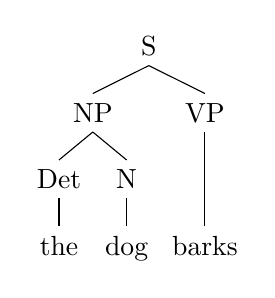
\begin{tikzpicture}
\tikzset{level 1+/.style={level distance=2\baselineskip}}
\tikzset{frontier/.style={distance from root=6\baselineskip}}
\Tree[.S
       [.NP 
         [.Det the ]
         [.N   dog ] ]
       [.VP barks ] ]
\end{tikzpicture}
}
\caption{\label{fig-the-dog-barks}Tree for \emph{The dog barks.} drawn with \texttt{tikz-qtree}}
\end{figure}
\begin{fitverb}
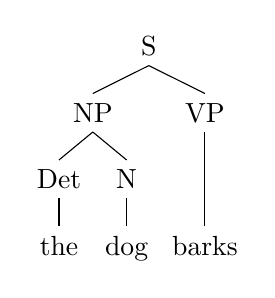
\begin{tikzpicture}
\tikzset{level 1+/.style={level distance=2\baselineskip}}
\tikzset{frontier/.style={distance from root=6\baselineskip}}
\Tree[.S
       [.NP 
         [.Det the ]
         [.N   dog ] ]
       [.VP barks ] ]
\end{tikzpicture}
\end{fitverb}

The code below shows how words below a certain node can be put under a triangle as in Figure~\vref{fig-the-dog-barks-abbreviated}.
\begin{figure}[htbp]
\centerline{%
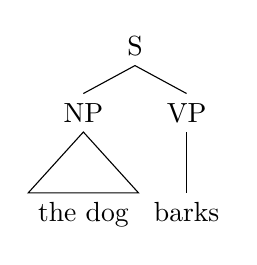
\begin{tikzpicture}
\tikzset{level 1+/.style={level distance=2\baselineskip}}
\tikzset{frontier/.style={distance from root=5\baselineskip}}
\Tree[.S
       [.NP  \edge[roof]; {the dog} ]
       [.VP barks ] ]
\end{tikzpicture}
}
\caption{\label{fig-the-dog-barks-abbreviated}Tree for \emph{The dog barks.} with abbreviated NP}
\end{figure}

\begin{samepage}
\begin{fitverb}
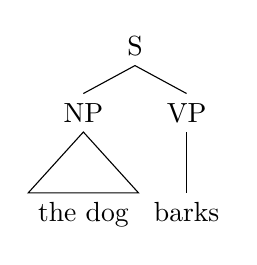
\begin{tikzpicture}
\tikzset{level 1+/.style={level distance=2\baselineskip}}
\tikzset{frontier/.style={distance from root=5\baselineskip}}
\Tree[.S
       [.NP  \edge[roof]; {the dog} ]
       [.VP barks ] ]
\end{tikzpicture}
\end{fitverb}
\end{samepage}
\ispackagee{tikz-qtree} 

\subsection{DRSes: \texttt{drs}}

DRSes\ispackageb{drs} can be typeset using the \texttt{drs} package by Alexis Dimitriadis\aimention{Alexis
  Dimitriadis}. There are various commands that let you typeset simple DRSes, ones with implications
and DRSes with quantifiers. Some examples from the manual are given below:

\bigskip

\drs{x y}{Jones(x) \\ Ulysses(y) \\ x owns y}

\begin{verbatim}
\drs{x y}{Jones(x) \\ Ulysses(y) \\ x owns y}
\end{verbatim}


\drs{x}{Jones(x) \\
      \ifdrs{y}{donkey(y)\\x owns y}
            {z w}{z = x\\ w = y\\ z feeds w}}

\begin{verbatim}
\drs{x}{Jones(x) \\
      \ifdrs{y}{donkey(y)\\x owns y}
            {z w}{z = x\\ w = y\\ z feeds w}}
\end{verbatim}

\drs{X}{ the lawyers(X) \\
        \qdrs{x}{x $\in$ X}
             {every}{x}
             {y}{secretary(y) \\ x hired y}}

\begin{verbatim}
\drs{X}{ the lawyers(X) \\
        \qdrs{x}{x $\in$ X}
             {every}{x}
             {y}{secretary(y) \\ x hired y}}
\end{verbatim}
\ispackagee{drs}

%%%%%%%%%%%%%%%%%%%%%%%%%%%%%%%%%%%%%%%%%%%%%%%%%%%%%%%%%%%%%%%%%%%%%%%%%%%%%%%%%%%%%%%%%%%%%%%%%%%

\subsection{AVMs}

\ispackageb{avm}
  \begin{avm}
    {\it word\/} $\rightarrow$
    \[morphs & $\@{e_1}\bigcirc\cdots\bigcirc\@{e_n}$\\
    morsyn & \@0 $(\@{m_1}\uplus\cdots\uplus\@{m_n})$\\
    rules & \< \[morphs & \@{e_1}\\mud & \@{m_1}\\ morsyn & \@0\],\ldots,
    \[morphs & \@{e_n}\\mud & \@{m_n}\\ morsyn & \@0\] \>
    \]
  \end{avm}
\ispackagee{avm}

\subsection{OT tableaux}


This\is{Optimality Theory|(}\is{tabular} section just provides some examples of how Optimality Tableaux can be typeset.

\begin{tabular}
       {|lc|c|c|c|}\hline   
      & \textbf{Input}  & Cnstrnt 1  &  Cnstrnt 2& Cnstrnt 3\\ \hline\hline
      & candidate 1     & *!         &           &          \\ \hline
      & candidate 2     &            &  *        &          \\ \hline
\hand & candidate 3     &            &           &  *       \\ \hline
\end{tabular}

\begin{fitverb}
\begin{tabular}
       {|lc|c|c|c|}\hline   
      & \textbf{Input}  & Cnstrnt 1  &  Cnstrnt 2& Cnstrnt 3\\ \hline\hline
      & candidate 1     & *!         &           &          \\ \hline
      & candidate 2     &            &  *        &          \\ \hline
\hand & candidate 3     &            &           &  *       \\ \hline
\end{tabular}
\end{fitverb}

\verb+\hand+ is defined as follows:

\begin{verbatim}
\usepackage{pifont}
\newcommand{\hand}{\ding{43}}
\end{verbatim}
 


\begin{tabular*}{0.95\textwidth}
    {@{\extracolsep{\fill}}|rl||c|c|c|}\hline   
      & \textbf{Input} & Constraint 1 & Constraint 2 & Constraint 3 \\ \hline\hline
      & candidate 1    & *!           &              &              \\ \hline
      & candidate 2    &              &  *           &              \\ \hline
\hand & candidate 3    &              &              &  *           \\ \hline
\end{tabular*}

\begin{fitverb}
\begin{tabular*}{0.95\textwidth}
    {@{\extracolsep{\fill}}|rl||c|c|c|}\hline   
      & \textbf{Input} & Constraint 1 & Constraint 2 & Constraint 3 \\ \hline\hline
      & candidate 1    & *!           &              &              \\ \hline
      & candidate 2    &              &  *           &              \\ \hline
\hand & candidate 3    &              &              &  *           \\ \hline
\end{tabular*}
\end{fitverb}

\begin{tabular}[t]{r|c|c|c|}
\cline{2-4}
      & /qi/  & qi    & qi         \\
\LCC 
      &       &       & \lightgray \\ \cline{2-4}
\hand & [qi]  &       & *          \\ \cline{2-4}
      & [*qi] & *!    &            \\ \cline{2-4}
\ECC
\end{tabular}


\begin{verbatim}
\usepackage{pstricks,colortab}

\begin{tabular}[t]{r|c|c|c|}
\cline{2-4}
      & /qi/  & qi    & qi         \\
\LCC 
      &       &       & \lightgray \\ \cline{2-4}
\hand & [qi]  &       & *          \\ \cline{2-4}
      & [*qi] & *!    &            \\ \cline{2-4}
\ECC
\end{tabular}
\end{verbatim}


\begin{tabular}{|l||c|c|} \hline
          &VO          &OV         \\ \hline\hline
\LCC
          &            &\lightgray \\ \hline
prefixing &Tagalog     &Ma'a       \\ \hline
\ECC
\LCC
           &\lightgray &            \\ \hline
suffixing  &Kwakwala   &Japanese    \\ \hline
\ECC
\end{tabular}

\begin{verbatim}
\begin{tabular}{|l||c|c|} \hline
          &VO          &OV         \\ \hline\hline
\LCC
          &            &\lightgray \\ \hline
prefixing &Tagalog     &Ma'a       \\ \hline
\ECC
\LCC
           &\lightgray &            \\ \hline
suffixing  &Kwakwala   &Japanese    \\ \hline
\ECC
\end{tabular}
\end{verbatim}
\is{Optimality Theory|)}



\subsection{Font issues and right to left scripts}

Since\is{font|(} we are using \xelatex, all fonts that are installed in the cannonical font directories can be
used. We are using the font \texttt{Linux Libertine}, which is unicode-based and contains a lot of
the characters linguists want to use.

\subsubsection{Chinese}
\label{sec-Chinese}

You can enter Chinese\il{Chinese}\is{Chinese Characters} characters directly and mix them with ASCII text without any further markup
provided you load the \texttt{xeCJK}\ispackage{xeCJK} package. We already saw an example in (\ref{ex-chinese}) on
page~\pageref{ex-chinese}. In order to type Chinese text, one has to load the \texttt{xeCJK} package
with the option \verb+indentfirst+ set to \verb+false+ and select an appropriate font:
\begin{verbatim}
\usepackage[indentfirst=false]{xeCJK}
\setCJKmainfont{SimSun}
\end{verbatim}


\subsubsection{Arabic script}

Arbaic script\is{Arabic Script}\il{Persian} is the most challenging script for typesetting since it is written from right to left
and contains ligatures. If you load the \texttt{bidi} package, you can mix right to left and left to
right text.\footnote{
  Please have a look at the source code. The verbatim environment has difficulties to display Arabic
  text and hence the call to \texttt{$\backslash$PRL} comes out scrambled.
}

\ea
\PRL{او مرد را دوست نخواهد داشت.}\\

\PRL{او مرد را دوست نخواهد داشت. و مرد را دوست نخواهد داشت. و مرد را دوست نخواهد داشت. و مرد را دوست نخواهد داشت.}\\
 \gll U      mard rā        dust   naxāhad        dāšt.\\
      He/she man  {\sc dom} friend {\sc neg}.want have\\
\glt `He/she will not love the man.'
\z

%\begin{rtlverbatim}
%\usepackage{fontspec}
\begin{verbatim}
\newfontfamily\Parsifont[Script=Arabic]{XB Niloofar}
\usepackage{bidi}
\newcommand{\PRL}[1]{\RL{\Parsifont #1}}

\ea
\PRL{او مرد را دوست نخواهد داشت.}\\
\gll U      mard rā       dust   naxāhad        dāšt.\\
     He/she man {\sc dom} friend {\sc neg}.want have\\
\glt `He/she will not love the man.'
\z
\end{verbatim}
%\end{rtlverbatim}

\subsubsection{Hebrew}

Hebrew\il{Hebrew|(} is also written from right to left. The characters are part of Linux Libertine, so no extra
font has to be loaded to set examples like (\mex{1}):
\ea
\glll \RL{האישה קוראת ספר.}\\
       ha-'iša          qore't	                          sefer.\\
       {\sc def}-woman  read.{\sc pres}.{\sc f}.{\sc sg}  book\\
\glt `The woman is reading a book.'
\z
\begin{fitverb}
\ea
\glll \RL{האישה קוראת ספר.}\\
       ha-'iša          qore't                            sefer.\\
       {\sc def}-woman  read.{\sc pres}.{\sc f}.{\sc sg}  book\\
\glt `The woman is reading a book.'
\z
\end{fitverb}
\il{Hebrew|)}

\subsubsection{IPA symbols}

The\is{IPA symbols|(} IPA symbols are part of the Linux Libertine font and hence can be entered into the document
directly. The IPA unicode symbols can be created online at
\url{http://ipa.typeit.org/full/}. (\mex{1}) shows some examples:
\ea
ɓ ɐ ʁ ɾ ɻ ʃ ʂ θ~  t͡ʃ~  t͡s  ʈ ʊ ʊ̈ ʉ ʌ ʋ ʍ ɯ ɰ χ ʎ ɣ ʏ ɤ ʒ ʐ ʑ ʔ ʕ ʢ ʡ ɑ̃ ɔ ˧ ˨ ˩ ˩˥ ˥˩ ˦˥
\z
% ⱱ does not work  
If you find symbols that are not covered by the font, please use the \texttt{tipa} package.
\is{font|)}\is{IPA symbols|)}

\section{Bells and whistles}

\subsection{\texttt{varioref}}

\texttt{varioref}\ispackageb{varioref} is loaded by the \lsp class file. You can use \verb+\vref+\iscommand{vref} to refer to floating
objects like figures and tables. \latex automatically determines whether the floating object is on
the same page or further away. If the float is on the next page and the next page is to the right of
the current page, \latex will insert an appropriate text like \emph{on the facing page}. If we are
on a right page, \latex will insert something like \emph{on the next page} or \emph{on the facing page}. If the float is further
away, a page number will be provided.
\ispackagee{varioref}

%Please use \verb+\vref+ for the first reference to a float only.


\subsection{\texttt{german} for hyphenation}

If\is{hyphenation|(}\ispackageb{german} you write things like \verb+head-driven+ or very long pathes like
{\sc snysem$|$""loc$|$""cat$|$""head$|$""mod$|$""loc}, \LaTeX{} does not do hyphenation
(in the part following the dash).

\verb+german.sty+ provides additional markup that allows for proper hyphenation:
\begin{verbatim}
head"=driven

{\sc snysem$|$""loc$|$""cat$|$""head$|$""mod$|$""loc}
\end{verbatim}
With this markup even long pathes like {\sc snysem$|$loc$|$cat$|$""head$|$""mod$|$""loc$|$""cat$|$""head}
are typeset properly. Alternatively you my write
\begin{verbatim}
{\sc snysem$|$\-loc$|$\-cat$|$\-head$|$\-mod}
\end{verbatim}
which introduces a dash at the place of the linebreak:
{\sc snysem$|$\-loc$|$\-cat$|$\-head$|$\-mod$|$\-loc$|$\-cat$|$\-head}.

If you use \verb+german.sty+ for a book whose primary language is not German, do not forget to
specify the language you are using. For example, if your book is in US English you have to specify
the following:
\begin{verbatim}
\selectlanguage{USenglish}
\end{verbatim}
Otherwise the section name for references comes out in German.
\is{hyphenation|)}\ispackagee{german}

\subsection{Resizing large objects}

Trees and AVMs often are too big to fit onto one page. The \texttt{langsci} comes with commands for
shrinking large objects. You may pass your complex object as an argument to \texttt{\oneline} and
this will scale the object to \verb+\linewidth+ (the remaining space on the current line). There is
a more clever version of this command: \verb+\centerfit+. This command checks whether there is
enough space for an object and if this is the case it centers it in the line. If the object is
larger than the \verb+\linewidth+, it is resized to fit the line. This is very handy for typesetting
figures. You may copy and paste figures to other documents with a different text width without any
adaptions.


%% \begin{figure}[htb]
%% \centerfit{%
%% \begin{tikzpicture}
%% \tikzset{level 1+/.style={level distance=3\baselineskip}}
%% \tikzset{level 2+/.style={level distance=5\baselineskip}}
%% \tikzset{level 3+/.style={level distance=6\baselineskip}}
%% \tikzset{level 4/.style={level distance=7\baselineskip}}
%% \tikzset{level 5+/.style={level distance=5\baselineskip}}
%% \tikzset{frontier/.style={distance from root=26\baselineskip}}
%% %% \Tree[.{\ms[np-passive-cx]{ vform & passive \\
%% %%                             subj & \sliste{ NP\ind{1} }\\[2mm]
%% %%                             comps & \sliste{ (PP[\type{by}]\ind{2}) }\\
%% %%                           } }
%% %%         \ms{ vform & psp \\
%% %%              subj & \sliste{ NP\ind{2} }\\[2mm]
%% %%              comps & \sliste{ NP\ind{1} } 
%% %%            } ]
%% \Tree[.S
%%        [.{\ibox{1} NP\ind{2}} \edge[roof]; {the boy} ]
%%        [.VP\feattab{
%%                  \subj  \sliste{ \ibox{1} NP\ind{2} },\\
%%                  \comps  \sliste{  }}
%%          [.V\feattab{
%%                  \subj  \sliste{ \ibox{1} NP\ind{2} },\\
%%                  \comps  \sliste{ \ibox{3} }} was ]
%%          [.{\ibox{3} VP\feattab{
%%                  \vform \type{passive},\\
%%                  \subj  \sliste{ \ibox{1} NP\ind{2} },\\
%%                  \comps  \sliste{ }}} \edge node[auto=left]{Passive Construction};
%%            [.V\feattab{
%%                  \vform \type{psp},\\
%%                  \subj  \sliste{ NP },\\
%%                  \comps  \sliste{ NP\ind{2} }} 
%%              [.V\feattab{
%%                  \vform \type{psp},\\
%%                  \subj  \sliste{ NP },\\
%%                  \comps  \sliste{ NP\ind{2}, \ibox{4} }} given ] \edge node[auto=left]{Schema for Passive Participles};
%%              [.{\ibox{4} NP} \edge[roof]; { the ball } ] ] ] ] ] 
%% \end{tikzpicture}
%% }
%% \caption{\label{fig-the-boy-was-given-the-ball-tseng}Analysis of \emph{The boy was given the ball} according to \citet{Tseng2007a}}
%% \end{figure}


\subsection{Rotating figures and tables}
 

\subsection{\texttt{xspace} and abbreviations}

\ispackage{xspace}

\subsection{\texttt{todonotes}}

\ispackage{todonotes}

%% \section{Software}

%% \begin{itemize}
%% \item BibDesk
%% \item JabRef
%% \end{itemize}


\subsection{Style files and multiple projects}

Pathes, shell variables \ldots

\section{Things you should not do}

Please do not use explicit linebreaks to mark a new paragraph. Paragraphs are marked by an empty
line in the text.

\section{Checklist for typesetters/authors using \latex}
\label{sec-check-typesetters}


%      <!-- Local IspellDict: en_US-w_accents -->

%% -*- coding:utf-8 -*-
\chapter{Publication}

Language Science Press books are published on the Document Server of the Freie Universität Berlin
together with a Print on Demand option.



Authors have to sign a publication contract with the FU Library. The contract is availible here in
German:
\url{http://edocs.fu-berlin.de/docs/content/main/autoren/vertraege.xml?XSL.lastPage.SESSION=/content/main/autoren/vertraege.xml&lang=en}. This
German contract has to be signed, but there is an English translation of it for reference.


Authors have to make sure that they have permission to use copyrighted material from journals or
other books. A respective declaration is part of the contract with the FU Library.




\backmatter

\bibliography{lsp-abbrev,lsp-guidelines}

%\cleardoublepage

\clearpage
\pdfbookmark[0]{Index}{Index}
\pdfbookmark[1]{Index of Names}{Index of Names}
\printindex[aut]
%\addcontentsline{toc}{chapter}{Verzeichnis der Sprachen}
\pdfbookmark[1]{Index of Languages}{Index of Languages}
\printindex[lan]
%\addcontentsline{toc}{chapter}{Sachregister}
\pdfbookmark[1]{Index of Subjects}{Index of Subjects}
\printindex

                              
\end{document}
      
%      <!-- Local IspellDict: en_US-w_accents -->
